\documentclass[runningheads]{llncs}

\usepackage[T1]{fontenc}
\usepackage{graphicx}
\usepackage{booktabs}
\usepackage{url}
\usepackage{amsmath}
\usepackage{amssymb}
\usepackage{array}
\usepackage{tabularx}
\usepackage{hyperref}
\usepackage{tikz}
\usetikzlibrary{arrows.meta,positioning,shapes.geometric,fit,backgrounds}

\begin{document}

\title{Privacy by Design in AI-Assisted Cybersecurity Policy
Generation: Benchmarking Private RAG Against Frontier AI Models}

\titlerunning{Privacy by Design in AI-Assisted Policy Generation}

\author{VV.AA.}
\authorrunning{VV.AA.}
\institute{The Lisbon Council, Brussels, Belgium}

\maketitle

\begin{abstract}
% TODO: write abstract last
Lorem ipsum dolor sit amet, consectetur adipiscing elit. Sed do eiusmod
tempor incididunt ut labore et dolore magna aliqua. Ut enim ad minim
veniam, quis nostrud exercitation ullamco laboris nisi ut aliquip ex ea
commodo consequat. Duis aute irure dolor in reprehenderit in voluptate
velit esse cillum dolore eu fugiat nulla pariatur. Excepteur sint occaecat
cupidatat non proident, sunt in culpa qui officia deserunt mollit anim id
est laborum.
\end{abstract}

\keywords{cybersecurity policy generation \and large language models \and
retrieval-augmented generation \and GDPR compliance \and
privacy-preserving AI \and LLM evaluation}


% -----------------------------------------------------------------------
\section{Introduction}
% -----------------------------------------------------------------------

The NIS2 Directive~\cite{nis22022} extends mandatory cybersecurity
obligations to over 160,000 organisations across the EU --- healthcare,
energy, transport, public administration, defence supply chains --- many of
which previously operated without formal information security policies.
Combined with GDPR~\cite{gdpr2016} and the AI Act~\cite{aiact2024}, regulated
organisations now face a growing policy compliance gap: the legal requirement
to produce, maintain, and audit cybersecurity policy artefacts has outpaced
the internal capacity to create them. The burden falls hardest on
resource-constrained organisations --- a regional hospital with a single IT
manager, a small NATO support unit without a dedicated CISO --- for which
producing context-specific, regulation-aligned policies from scratch
represents a prohibitive cost in both expertise and time.

Frontier AI models offer a compelling response: scalable, on-demand access
to expertise that would otherwise require external consultants.
The effectiveness of AI-assisted policy generation has begun to be
validated~\cite{mcintosh2023harnessing,jawhar2024aibased}. Yet effective
policy generation is not a one-shot task. A policy that does not reflect the
organisation's actual asset inventory, threat model, regulatory regime, and
operational constraints is at best a template and at worst a compliance
artefact that conveys false assurance. Context-elicitation --- a structured
dialogue that gathers organisational specifics before drafting --- is
therefore essential to output quality.

Here lies a fundamental tension. The data required to generate a useful
policy is by definition sensitive: organisational structure, known
vulnerabilities, gap analyses, incident history, cloud footprint. Under
GDPR Arts~28, 32, and 44--49~\cite{gdpr2016}, organisations in regulated
sectors cannot route this data through processors without an adequate Data
Processing Agreement (DPA), let alone across extra-EU boundaries without a
transfer mechanism. A healthcare provider generating its data protection
policy through a consumer-tier frontier assistant is, structurally, already
in violation of the regime the policy is meant to implement. The industry
has responded with two patterns: cloud RAG on proprietary providers
(OpenAI Assistants, Azure OpenAI) --- which improves grounding but does not
address EU data residency, open-weight portability, or DPA; and private RAG
on EU-resident open-weight models --- which addresses all three. Yet no
prior study evaluates output quality and privacy compliance of the
underlying inference architecture simultaneously under the same evaluation
rubric. Figure~\ref{fig:arch} illustrates the three architectural patterns
and their respective EU data perimeters.

\begin{figure}[t]
\centering
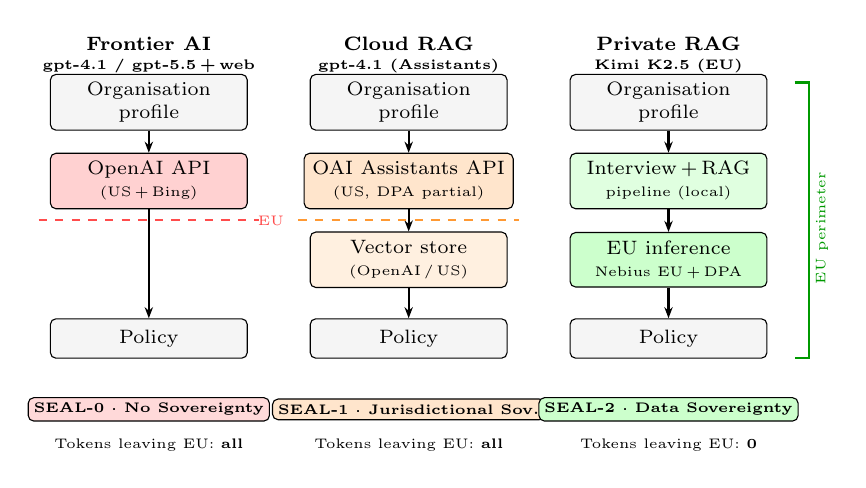
\begin{tikzpicture}[
  cbox/.style={draw, rounded corners=2pt, minimum width=2.5cm,
               minimum height=0.5cm, font=\scriptsize, align=center,
               inner sep=3pt},
  arr/.style={-{Stealth[length=4pt]}, thick},
  lbl/.style={font=\scriptsize\bfseries, align=center},
  seal/.style={draw, rounded corners=2pt, minimum width=2.5cm,
               font=\tiny\bfseries, align=center, inner sep=2pt},
]

%% ---- Column spacing
\def\ca{0}   % frontier
\def\cb{3.3} % cloud RAG
\def\cc{6.6} % private RAG

%% ---- Row heights (top to bottom)
\def\rA{4.4}  % org input
\def\rB{3.4}  % API / pipeline
\def\rC{2.4}  % storage / inference
\def\rD{1.4}  % output
\def\rS{0.5}  % SEAL badge

%% ======== COLUMN 1 — Frontier AI ========
\node[lbl] at (\ca,5.0) {Frontier AI\\[-1pt]{\tiny gpt-4.1 / gpt-5.5\,+\,web}};
\node[cbox, fill=gray!8]  (c1org) at (\ca,\rA) {Organisation\\profile};
\node[cbox, fill=red!18]  (c1api) at (\ca,\rB) {OpenAI API\\{\tiny (US\,+\,Bing)}};
\node[cbox, fill=gray!8]  (c1out) at (\ca,\rD) {Policy};

\draw[arr] (c1org) -- (c1api);
\draw[arr] (c1api) -- ++(0,-0.55) -- (c1out.north);

% EU boundary line — crossed by arrow
\draw[dashed, red!70, thick] (-1.4,2.9) -- (1.4,2.9);
\node[font=\tiny, red!70] at (1.55,2.9) {\rotatebox{0}{EU}};

\node[seal, fill=red!15] at (\ca,\rS) {SEAL-0 · No Sovereignty};

%% ======== COLUMN 2 — Cloud RAG ========
\node[lbl] at (\cb,5.0) {Cloud RAG\\[-1pt]{\tiny gpt-4.1 (Assistants)}};
\node[cbox, fill=gray!8]   (c2org) at (\cb,\rA) {Organisation\\profile};
\node[cbox, fill=orange!20](c2api) at (\cb,\rB) {OAI Assistants API\\{\tiny (US, DPA partial)}};
\node[cbox, fill=orange!12](c2vs)  at (\cb,\rC) {Vector store\\{\tiny (OpenAI\,/\,US)}};
\node[cbox, fill=gray!8]   (c2out) at (\cb,\rD) {Policy};

\draw[arr] (c2org) -- (c2api);
\draw[arr] (c2api) -- (c2vs);
\draw[arr] (c2vs)  -- (c2out);

\draw[dashed, orange!80, thick] (1.9,2.9) -- (4.7,2.9);

\node[seal, fill=orange!20] at (\cb,\rS)
  {SEAL-1 · Jurisdictional Sov.};

%% ======== COLUMN 3 — Private RAG ========
\node[lbl] at (\cc,5.0) {Private RAG\\[-1pt]{\tiny Kimi K2.5 (EU)}};
\node[cbox, fill=gray!8]   (c3org) at (\cc,\rA) {Organisation\\profile};
\node[cbox, fill=green!12] (c3int) at (\cc,\rB) {Interview\,+\,RAG\\{\tiny pipeline (local)}};
\node[cbox, fill=green!20] (c3inf) at (\cc,\rC) {EU inference\\{\tiny Nebius EU\,+\,DPA}};
\node[cbox, fill=gray!8]   (c3out) at (\cc,\rD) {Policy};

\draw[arr] (c3org) -- (c3int);
\draw[arr] (c3int) -- (c3inf);
\draw[arr] (c3inf) -- (c3out);

% No EU boundary crossed — green bracket on the right
\draw[green!60!black, thick] (8.2,\rA+0.25) -- ++(0.18,0) --
  ++(0,-\rA+\rD-0.5) -- ++(-0.18,0);
\node[font=\tiny, green!60!black, rotate=90] at (8.55, 2.8) {EU perimeter};

\node[seal, fill=green!20] at (\cc,\rS)
  {SEAL-2 · Data Sovereignty};

%% ---- Tokens-leave-EU row labels (very small, below SEAL)
\node[font=\tiny, align=center] at (\ca, 0.05)
  {Tokens leaving EU: \textbf{all}};
\node[font=\tiny, align=center] at (\cb, 0.05)
  {Tokens leaving EU: \textbf{all}};
\node[font=\tiny, align=center] at (\cc, 0.05)
  {Tokens leaving EU: \textbf{0}};

\end{tikzpicture}
\caption{The three architectural patterns benchmarked in this study.
  Dashed lines mark where data crosses the EU perimeter; the green bracket
  in the Private RAG column indicates that no data leaves the EU perimeter.
  SEAL levels follow the EC Cloud Sovereignty Framework~\cite{ecseal2026}.}
\label{fig:arch}
\end{figure}

\textbf{Research question:} \textit{Does a well-architected private RAG
system (EU-region + DPA + open-weight) produce cybersecurity policies of
comparable or superior quality to frontier AI models, while remaining
GDPR-compliant by construction?}

We address this question by contributing: (i)~an empirical benchmark
comparing six AI configurations on 60 policy generation tasks in two
regulated contexts; (ii)~a controlled pairwise ablation for backbone
selection within the same RAG architecture; and (iii)~a joint quality-and-privacy
evaluation framework applicable to regulated deployment contexts.


% -----------------------------------------------------------------------
\section{Related Work}
% -----------------------------------------------------------------------

LLM-based cybersecurity policy generation is an emerging area.
McIntosh et al.~\cite{mcintosh2023harnessing} demonstrated that GPT-4 can
generate GRC policies that outperform human-written ones in certain
ransomware mitigation contexts; the study relies on human moderation and
legal expert oversight throughout — an implicit acknowledgement that data
handling risks are unresolved. Jawhar et al.~\cite{jawhar2024aibased}
similarly demonstrate AI effectiveness for security policy and procedure
drafting without addressing GDPR or data residency constraints. In both
cases, quality is assessed informally without a replicable evaluation
rubric, and no privacy-compliant architecture is tested.

LLM-as-judge methodology provides the evaluation backbone for our
study~\cite{anthropic2024demystifying}. Zheng et al.~\cite{zheng2023judging}
demonstrate that GPT-4 as a judge reaches over 80\% agreement with human
experts on instruction-following tasks; positional and verbosity biases can be
partially mitigated by swapping answer positions and using chain-of-thought
prompting. Liu et al.~\cite{liu2023geval} introduce G-Eval, a form-filling
framework with probability-weighted scoring that correlates more strongly with
human judgement than string-overlap metrics. Human calibration of automated
rubrics is typically quantified via Cohen's~$\kappa$; Dubois et
al.~\cite{dubois2023alpacafarm} provide a methodological baseline for this
calibration step in the context of preference evaluation.

The deployment of AI for cybersecurity policy generation in regulated
organisations raises privacy constraints that go beyond GDPR surface
compliance. Two distinct properties must be distinguished:
\textit{data residency} — the physical location of storage and processing,
including logs, backups, and telemetry — and \textit{data sovereignty} — the
legal jurisdiction governing the provider and its sub-processor
chain~\cite{gdpr2016,schremsii2020}. A provider incorporated outside the EU
may retain legal exposure even when operating EU-located servers: the US
Clarifying Lawful Overseas Use of Data Act (CLOUD Act)~\cite{cloudact2018}
permits US authorities to compel disclosure of data held by US-incorporated
entities regardless of physical location. An additional risk vector is the
sub-processor chain: a provider with EU legal domicile may add an extra-EU
sub-processor unilaterally, extending the exposure perimeter without customer
notification~\cite{gdpr2016}. Existing benchmarks of AI-assisted
cybersecurity policy generation~\cite{mcintosh2023harnessing,jawhar2024aibased}
evaluate output quality in isolation; to our knowledge, no prior work
simultaneously evaluates output quality and the privacy compliance of the
underlying inference architecture within a unified framework.


% -----------------------------------------------------------------------
\section{Methodology}
% -----------------------------------------------------------------------

\subsection{Experimental Design}

The study adopts a two-phase design. In the first phase, a backbone
selection experiment compares two open-weight models running on an
identical private RAG architecture, in order to select the stronger
candidate before the full benchmark. In the second phase, the selected
private RAG configuration is benchmarked against four frontier AI
configurations spanning the design space from unaugmented chat to
cloud-hosted RAG.

All policy artefacts are generated from synthetic organisational profiles
designed to represent typical regulated-sector environments (see
Section~\ref{sec:setup}). The use of synthetic data allows full control
over the experimental conditions and avoids any real data privacy concern
in the evaluation pipeline itself.

\subsection{Policy Generation}

Each artefact is produced through a multi-turn adaptive interview. The
system conducts 6--8 dialogue turns gathering organisational context
(sector, size, regulatory regime, existing controls, cloud footprint), then
generates the full policy document in a single final turn. The private RAG
configurations augment this generation with retrieval from a curated
knowledge base of 837~chunks drawn from NIST CSF~2.0, ISO/IEC~27001:2022,
GDPR, NIS2, the AI Act, and sector-specific guidance for healthcare and
defence. Frontier configurations either use no augmentation or rely on
live web search.

\subsection{Evaluation Framework}
\label{sec:grader}

Each artefact is evaluated by an LLM-as-judge pipeline using Claude
Opus~4.7 as the scoring model, following the structured grader blueprint
described in~\cite{anthropic2024demystifying}. The judge receives three
inputs: the generated policy, the synthetic organisational profile used
during generation, and a detailed scoring rubric. It returns a score from
1 to~5 on each of seven quality dimensions (see Section~\ref{sec:rubric}),
accompanied by a brief scoring rationale.

The rubric combines objective checks — for example, presence of specific
regulatory citations or mandatory policy clauses — with holistic LLM-scored
assessments of coherence and contextual fit. This two-layer structure
reduces sensitivity to surface variation while preserving sensitivity to
substantive quality differences. Human calibration of the rubric against
subject-matter expert judgement (Cohen's~$\kappa$) is underway on a sample
of 6~artefacts and will be reported in the final version.

\paragraph{Rubric design rationale.}
The seven dimensions were derived in two steps. First, we mapped the
grading dimensions proposed by Anthropic for research
agents~\cite{anthropic2024demystifying} — groundedness of claims against
sources, coverage of key facts, source quality, and coherence of synthesis
— onto the policy generation task, yielding \textit{Evidence citation},
\textit{Content quality}, \textit{Source attribution}, and
\textit{Contextual adaptation} respectively. Second, we extended the rubric
with three dimensions specific to the cybersecurity compliance domain:
\textit{Regulatory alignment} (coverage of applicable regulatory
obligations, absent in generic agent evals); \textit{Implementability}
(actionability under real operational constraints); and
\textit{Resource consideration} (fitness for SME and public-sector
organisations where budget and staffing are primary constraints). The
extended rubric is publicly available with the evaluation code.
Figure~\ref{fig:grader} summarises the evaluation pipeline and the
derivation of the seven criteria.

\begin{figure}[t]
\centering
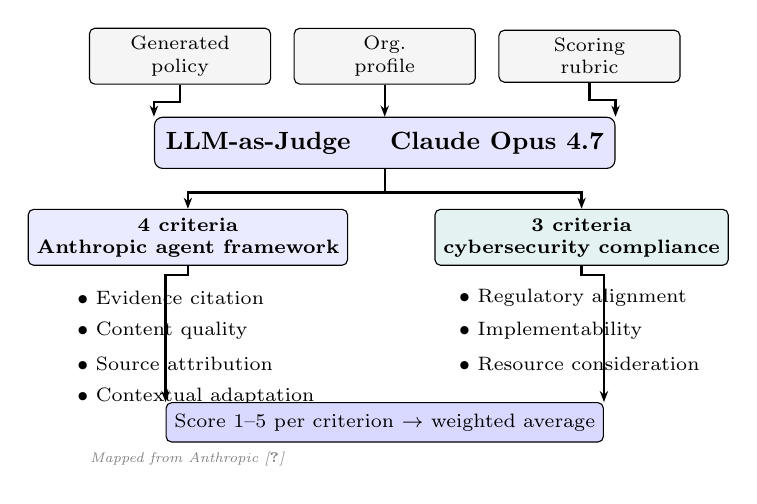
\begin{tikzpicture}[
  inp/.style={draw, rounded corners=2pt, fill=gray!8,
              minimum width=2.3cm, minimum height=0.5cm,
              font=\scriptsize, align=center, inner sep=3pt},
  judge/.style={draw, rounded corners=3pt, fill=blue!10,
                minimum width=5.0cm, minimum height=0.65cm,
                font=\small\bfseries, align=center, inner sep=4pt},
  grp/.style={draw, rounded corners=2pt, minimum width=3.2cm,
              font=\scriptsize\bfseries, align=center,
              inner sep=3pt, minimum height=0.55cm},
  crit/.style={draw=none, font=\scriptsize, align=left,
               inner sep=1pt, minimum height=0.42cm},
  arr/.style={-{Stealth[length=4pt]}, thick},
]

%% ---- Inputs (top row) ----
\node[inp] (pol) at (-2.6, 4.5) {Generated\\policy};
\node[inp] (pro) at (0,    4.5) {Org.\\profile};
\node[inp] (rub) at (2.6,  4.5) {Scoring\\rubric};

%% ---- Judge ----
\node[judge] (jdg) at (0, 3.4)
  {LLM-as-Judge \quad Claude Opus 4.7};

\draw[arr] (pol.south) -- ++(0,-0.22) -| (jdg.north west);
\draw[arr] (pro.south) -- (jdg.north);
\draw[arr] (rub.south) -- ++(0,-0.22) -| (jdg.north east);

%% ---- Two criterion groups ----
\node[grp, fill=blue!8]  (ga) at (-2.5, 2.2)
  {4 criteria\\Anthropic agent framework};
\node[grp, fill=teal!10] (gb) at (2.5, 2.2)
  {3 criteria\\cybersecurity compliance};

\draw[arr] (jdg.south) -- ++(0,-0.3) -| (ga.north);
\draw[arr] (jdg.south) -- ++(0,-0.3) -| (gb.north);

%% ---- Left criteria ----
\node[crit, anchor=north west] at (-3.95, 1.65) {$\bullet$~Evidence citation};
\node[crit, anchor=north west] at (-3.95, 1.23) {$\bullet$~Content quality};
\node[crit, anchor=north west] at (-3.95, 0.81) {$\bullet$~Source attribution};
\node[crit, anchor=north west] at (-3.95, 0.39) {$\bullet$~Contextual adaptation};

%% ---- Right criteria ----
\node[crit, anchor=north west] at (0.9, 1.65) {$\bullet$~Regulatory alignment};
\node[crit, anchor=north west] at (0.9, 1.23) {$\bullet$~Implementability};
\node[crit, anchor=north west] at (0.9, 0.81) {$\bullet$~Resource consideration};

%% ---- Score output ----
\node[inp, fill=blue!15, minimum width=4.5cm] (sc) at (0, -0.15)
  {Score 1--5 per criterion $\rightarrow$ weighted average};

\draw[arr] (ga.south) -- ++(0,-0.12) -| (sc.north west);
\draw[arr] (gb.south) -- ++(0,-0.12) -| (sc.north east);

%% ---- Source annotation ----
\node[font=\tiny, gray] at (-2.5, -0.62)
  {\textit{Mapped from Anthropic~\cite{anthropic2024demystifying}}};

\end{tikzpicture}
\caption{LLM-as-judge evaluation pipeline. Four criteria are mapped from
  the Anthropic research agent grading framework~\cite{anthropic2024demystifying};
  three are added for the cybersecurity compliance domain.}
\label{fig:grader}
\end{figure}


% -----------------------------------------------------------------------
\section{Experimental Setup}
\label{sec:setup}
% -----------------------------------------------------------------------

\subsection{Configurations}

We compared six configurations spanning the design space from
consumer-tier AI chat to privacy-compliant private RAG
(Table~\ref{tab:configs}).

\begin{table}[t]
\caption{Experimental configurations. GDPR compliance denotes the ability
to operate under GDPR Art.~28 (DPA), Art.~32 (security measures), and
Art.~44--49 (third-country transfers) as assessed from available
provider documentation. $\dagger$~OpenAI Assistants API provides a DPA
for API customers but does not guarantee EU data residency; data may be
processed under SCCs outside the EU.}
\label{tab:configs}
\small
\begin{tabular}{l c c l c}
\toprule
Model & \shortstack{Knowledge\\Base} & Web & Provider & GDPR \\
\midrule
gpt-4.1                          & --           & --           & OpenAI consumer    & $\times$ \\
gpt-4.1 + web search             & --           & \checkmark   & OpenAI + Bing      & $\times$ \\
gpt-5.5 + web search             & --           & \checkmark   & OpenAI + Bing      & $\times$ \\
gpt-4.1 (OpenAI Assistants RAG)  & \checkmark   & --           & OpenAI Assistants  & partial$^\dagger$ \\
Kimi K2.5 (private RAG)          & \checkmark   & --           & Nebius EU + DPA    & \checkmark \\
DeepSeek V3.2 (private RAG)      & \checkmark   & --           & Nebius EU + DPA    & \checkmark \\
\bottomrule
\end{tabular}
\end{table}

The first four configurations offer no EU data residency guarantee. The
private RAG configurations (Kimi K2.5 and DeepSeek V3.2) are
privacy-by-design: all inference runs within a Nebius EU region under a
DPA, using open-weight models whose weights can be independently audited.

\subsection{Backbone Selection}

Before the full benchmark, we compared Kimi K2.5 and DeepSeek V3.2 under
strictly identical conditions — same curated KB, identical system prompt,
same EU-region provider (Nebius), and no model-specific prompt tuning.
This controlled ablation isolates the backbone model as the sole variable,
ruling out architecture or prompt design as confounds.

\subsection{Evaluation Contexts and Policy Types}
\label{sec:rubric}

Each configuration was tested across two regulated contexts:
\textbf{ctx-H} (a small Italian public hospital, $\approx$200~staff,
subject to Italian healthcare regulations, NIS2, and GDPR) and
\textbf{ctx-M} (a NATO detachment in Romania, subject to NATO information
security policy). Five policy types were generated per context: Password
Policy, Data Protection Policy, Access Control Policy, Incident Response
Policy, and General Cybersecurity Policy, yielding 60~artefacts in total.

Each artefact was evaluated on seven quality dimensions
(Section~\ref{sec:grader}) with 1--5 Likert anchors:

\begin{enumerate}
  \item \textbf{Content quality:} accuracy and completeness of
        cybersecurity controls
  \item \textbf{Contextual adaptation:} fit to the specific
        organisational context
  \item \textbf{Evidence citation:} grounding in standards and
        regulatory sources
  \item \textbf{Implementability:} actionability and practical
        feasibility
  \item \textbf{Regulatory alignment:} coverage of applicable
        compliance requirements
  \item \textbf{Source attribution:} traceable references to cited
        sources
  \item \textbf{Resource consideration:} acknowledgement of
        organisational resource constraints
\end{enumerate}


% -----------------------------------------------------------------------
\section{Results}
% -----------------------------------------------------------------------

\subsection{Backbone Selection: Kimi K2.5 vs.\ DeepSeek V3.2}
\label{sec:backbone}

The pairwise judge returned 10/10 comparisons in favour of Kimi K2.5
over DeepSeek V3.2. Both models ran on the same private RAG architecture
with identical system prompt and KB; the result is attributable solely to
the models' differential ability to follow structured citation directives.
The gap is concentrated on normative traceability: source attribution
(4.10 vs.\ 2.30, $\Delta = 1.80$) and regulatory alignment
(4.20 vs.\ 2.90, $\Delta = 1.30$). Implementability is the sole dimension
where the models converge ($\Delta = 0.60$, 3~ties). Kimi K2.5 was
selected as the private RAG backbone for the full benchmark.

\subsection{Quality Scores Across Configurations}

Table~\ref{tab:results} reports mean scores across all ten artefacts per
configuration (two contexts $\times$ five policy types).
gpt-5.5 + web search achieves the highest average (4.60), followed by
Kimi K2.5 private RAG (4.15) and gpt-4.1 + web search (3.90).
The OpenAI Assistants RAG configuration falls below the no-RAG gpt-4.1
baseline on the overall average.

\begin{table}[t]
\caption{Mean quality scores by configuration (1--5 Likert scale). Bold:
highest value per row. DeepSeek V3.2 was eliminated after backbone
selection (Section~\ref{sec:backbone}) and is not included here.
Cost estimates based on average token counts from generation logs and
API list prices (May~2026). Latency: median wall-clock time, client-side.}
\label{tab:results}
\footnotesize
\begin{tabularx}{\linewidth}{X c c c c c}
\toprule
Dimension &
gpt-4.1 &
\shortstack{gpt-4.1\\+web} &
\shortstack{\textbf{gpt-5.5}\\+web} &
\shortstack{gpt-4.1\\(Asst.)} &
\shortstack{\textbf{Kimi}\\K2.5} \\
\midrule
Content quality        & 4.10 & 4.00 & \textbf{5.00} & 4.00 & 4.60 \\
Contextual adaptation  & 4.60 & 4.40 & \textbf{5.00} & 4.50 & \textbf{5.00} \\
Evidence citation      & 3.60 & 4.00 & \textbf{5.00} & 3.80 & 4.10 \\
Implementability       & 4.20 & 4.50 & \textbf{4.60} & 4.10 & 4.20 \\
Regulatory alignment   & 3.90 & 3.90 & \textbf{4.90} & 4.10 & 4.20 \\
Source attribution     & 4.20 & 4.50 & \textbf{4.50} & 3.80 & 4.10 \\
Resource consideration & 2.00 & 2.00 & \textbf{3.20} & 1.60 & \textbf{2.50} \\
\midrule
\textbf{Average}       & 3.83 & 3.90 & \textbf{4.60} & 3.70 & \textbf{4.15} \\
\midrule
Cost / query (USD)     & $\sim$0.02 & $\sim$0.03 & TBD & $\sim$0.07 & $\sim$0.05 \\
Latency (s)            & 33 & 30 & 278 & 41 & 36 \\
Tokens leaving EU      & all & all & all & all & \textbf{0} \\
\bottomrule
\end{tabularx}
\end{table}


\begin{figure}[t]
  \centering
  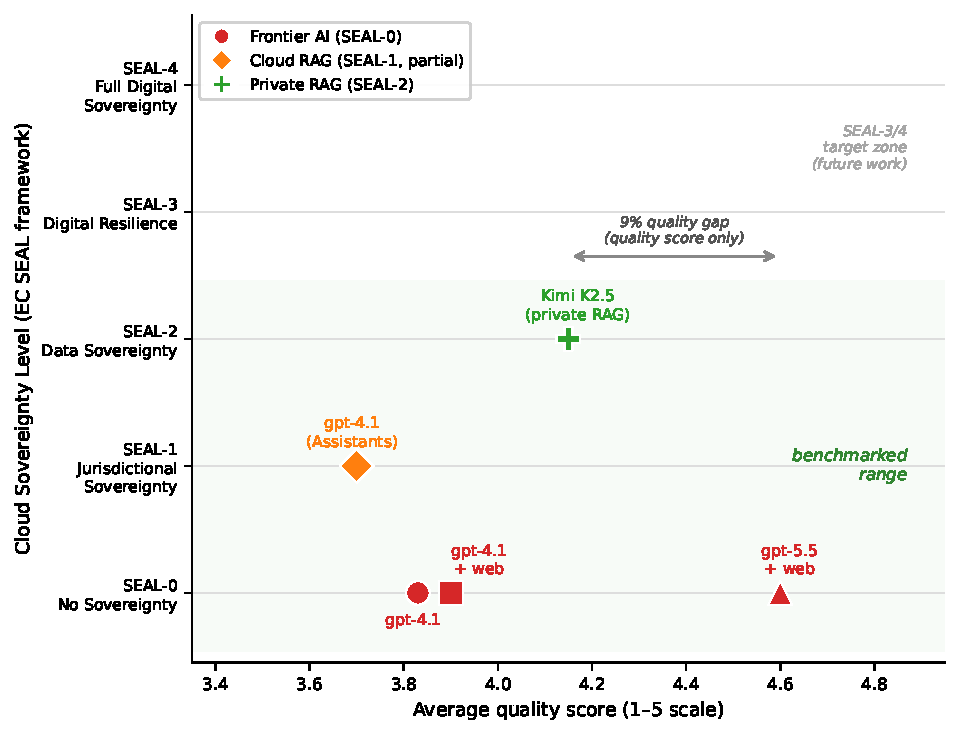
\includegraphics[width=0.92\linewidth]{figures/fig_scatter.pdf}
  \caption{Quality vs.\ privacy posture for the five benchmarked configurations.
    The 9\% quality gap between the best frontier configuration (gpt-5.5\,+\,web,
    avg.\ 4.60) and the private RAG configuration (Kimi K2.5, avg.\ 4.15)
    corresponds to a jump from SEAL-0 to SEAL-2 compliance.}
  \label{fig:scatter}
\end{figure}

% -----------------------------------------------------------------------
\section{Discussion}
% -----------------------------------------------------------------------

\subsection{Backbone Selection Within the Same RAG Architecture}

The 10/0 pairwise result and the per-dimension gap analysis establish that,
under equal conditions, Kimi K2.5 substantially outperforms DeepSeek V3.2
on dimensions requiring normative traceability. The concentration of the gap
on source attribution ($\Delta = 1.80$) and regulatory alignment
($\Delta = 1.30$) suggests that the two models differ in their ability to
follow structured citation directives — a finding that is independent of
prompt design, since both models received identical instructions.
Implementability ($\Delta = 0.60$, 3~ties) is the sole dimension where
the models converge, suggesting that general instruction-following is
comparable but domain-specific citation discipline is not.

A natural question is why the backbone selection did not include
Mistral~Large, the most capable EU-origin open-weight model at the time
of the experiments. The answer is methodological: the study benchmarks
the \emph{best available} open-weight candidate, not the most
sovereignty-compliant one. Including Mistral, whose preliminary
performance on the 7-criterion rubric was substantially lower, would
have artificially widened the quality gap and weakened the main thesis.
The reported 9\% gap between Kimi K2.5 and gpt-5.5\,+\,web is therefore
a conservative estimate: with a weaker backbone the gap would be larger.
Sovereignty and quality are orthogonal dimensions; the paper quantifies
both separately, and the path from SEAL-2 to SEAL-3 via a Mistral-based
backbone is identified as future work precisely because it carries a
quality cost that has not yet been empirically characterised.

\subsection{Frontier Benchmark Interpretation}

The 9\% quality gap between the best frontier configuration
(gpt-5.5 + web search, avg.\ 4.60) and the private RAG configuration
(Kimi K2.5, avg.\ 4.15) is concentrated in ctx-H, where the Italian
regulatory web corpus is rich and live web search provides substantive
grounding. The gap halves in ctx-M (NATO classified), precisely the context
where privacy posture matters most and where web search offers the least
domain-specific value.

The apparent advantage of gpt-5.5 + web search must be discounted by three
caveats: two processors without DPA (OpenAI and Bing), $10\times$ higher
cost, $7\times$ higher latency, and citations drawn from blogs and vendor
whitepapers rather than institutional sources. The audit trail of a private
RAG with a curated KB is deterministic and reproducible; the audit trail
of a frontier model with live web search is neither.

\textbf{[TODO: to be completed — add per-context breakdown (ctx-H vs
ctx-M); discuss OpenAI Assistants RAG underperformance; address
self-preference bias in LLM-as-judge.]}


% -----------------------------------------------------------------------
\section{Conclusion}
% -----------------------------------------------------------------------

For regulated organisations the question is not ``which model writes the
best policy'' but ``which architecture produces adequate policies under the
constraint that no data shall leave the perimeter.'' A private RAG on
EU-resident open-weight models is today a technically competitive option:
it achieves 90\% of frontier quality at one-tenth the cost, with full GDPR
compliance and a deterministic audit trail. The marginal quality gain
offered by frontier AI models does not justify the privacy cost they impose.

A further open question concerns the relative weight of two distinct
privacy properties: \textit{legal domicile} of the provider versus
\textit{physical residency} of the data. A provider legally incorporated
in the EU but operating sub-processors outside the EU may, in practice,
offer weaker GDPR protection than an EU-domiciled provider with a clean
sub-processor chain, even if the latter is less well-known. Conversely,
a non-EU provider (e.g., subject to the US CLOUD Act) that operates
servers exclusively in an EU region may offer strong data residency
guarantees while remaining legally exposed to extra-EU compelled
disclosure. Our experimental setup treats GDPR compliance as a binary
dimension assessed from published provider documentation; a more nuanced
analysis should evaluate the full sub-processor chain and the legal
jurisdiction of each entity in the inference path. We leave this as a
direction for future work.

These considerations are acquiring regulatory urgency. In April~2026 the
European Commission awarded its first procurement contract under the Cloud
Sovereignty Framework~\cite{ecseal2026}, which defines five Sovereignty
Effectiveness Assurance Levels (SEAL-0 to SEAL-4) and sets SEAL-2 as the
minimum threshold for EU institutional procurement. Under this framework,
frontier AI providers incorporated outside the EU qualify at SEAL-0 at best,
regardless of server location; all four winning consortia are EU-incorporated.
The private RAG architecture evaluated in this paper --- EU-resident open-weight
models under a DPA with an EU-incorporated provider --- aligns structurally
with SEAL-2 requirements, making the 9\% quality gap relative to the best
frontier configuration the operational cost of regulatory-grade sovereignty.
The adequacy basis underpinning US transfers, the EU--US Data Privacy
Framework~\cite{dpf2023}, meanwhile faces continued uncertainty: the General
Court upheld it in September~2025~\cite{latombe2025}, but the case is on
appeal before the CJEU, and the temporary loss of quorum of the Privacy and
Civil Liberties Oversight Board --- a structural redress pillar of the
framework --- illustrates the fragility of building long-term GDPR compliance
on executive-dependent mechanisms.
The GDPR and the CLOUD Act are therefore in structural, not episodic,
conflict~\cite{schremsii2020,cloudact2018}: two sovereign legal orders
asserting concurrent jurisdiction over the same data. The Cloud Sovereignty
Framework~\cite{ecseal2026} represents the first objective metric for
distinguishing verifiable legal sovereignty from superficial geographic
residency claims. For AI-assisted policy generation in regulated EU contexts,
a provider's SEAL level is a criterion complementary to, and arguably more
discriminating than, ISO/IEC~27001 certification or server location alone.

Several limitations bound the scope of this study. First, the evaluation
relies entirely on LLM-as-judge scoring; human expert calibration via
Cohen's~$\kappa$ is underway on a sample of artefacts and will be
reported in the extended version. Second, the benchmark covers two
organisational contexts (Italian public hospital and NATO detachment);
broader coverage across sectors and jurisdictions is needed to assess
generalisability. Third, cost estimates for gpt-5.5\,+\,web search are
preliminary pending stable API pricing.

A natural next step is to characterise the path from the current SEAL-2
private RAG architecture to SEAL-3. The binding constraint is the model
backbone: Kimi K2.5 is developed by Moonshot AI (China) and its weights
depend on an entity subject to the Chinese National Intelligence Law,
creating a residual non-EU supply-chain dependency. A SEAL-3 configuration
would require replacing the backbone with an EU-origin model --- Mistral
being the most mature candidate --- deployed on SEAL-3-certified
infrastructure (OVHcloud, STACKIT, or Scaleway), together with a locally
hosted embedding model to remove the remaining Nebius API call from the
retrieval pipeline. Notably, this requirement is not satisfied by Mistral's primary
commercial channels: API access via Microsoft Azure --- Mistral's
strategic distribution partner since 2024~\cite{azure_mistral2024} ---
is subject to CLOUD Act extraterritorial reach, whilst Mistral's own
managed platform (la.plateforme.ai) does not carry explicit SEAL-3
certification under the EC Cloud Sovereignty Framework~\cite{ecseal2026}.
EU-origin model selection and SEAL-3-certified deployment infrastructure
are therefore orthogonal requirements that must both be satisfied
independently.
Whether this full architectural upgrade preserves the
observed quality level relative to frontier systems is an open empirical
question.

Experimental code and generated policy artefacts will be released upon
publication to support reproducibility.

% -----------------------------------------------------------------------
\section*{Acknowledgements}
% -----------------------------------------------------------------------

This work has been carried out in the context of the COcyber project
(\textit{Coordination Between the Cybersecurity Civilian and Defence Spheres}),
funded by the European Union under the Horizon Europe programme,
Grant Agreement No.~101158606 (Call DIGITAL-ECCC-2023-DEPLOY-CYBER-04).
Views and opinions expressed are those of the authors only and do not
necessarily reflect those of the European Union or the European Cybersecurity
Competence Centre (ECCC). Neither the European Union nor the ECCC can be held
responsible for them.

\bibliographystyle{splncs04}
\bibliography{references}

\end{document}
